\documentclass[letter,twoside,11pt]{article}

\usepackage[spanish,es-nodecimaldot]{babel}
\usepackage[utf8]{inputenc}

\usepackage{lmodern}
\usepackage[T1]{fontenc}
\usepackage{textcomp}

\usepackage{framed}
\usepackage[svgnames]{xcolor}
\colorlet{shadecolor}{Gainsboro!50}

\usepackage[labelfont=bf]{caption}
\usepackage{graphicx}
\usepackage{pstricks}

\usepackage{anysize}
\marginsize{3cm}{2cm}{2cm}{3cm}

\usepackage{siunitx}
\usepackage{amsmath}
\usepackage{array}
\usepackage{csquotes}
\usepackage{amsfonts}

\usepackage{fancyhdr}
\usepackage{lastpage}
\pagestyle{fancy}
\fancyhf{}
\fancyhead[LE,RO]{Laboratorio de Electrónica Analógica I}
\fancyfoot[CO,CE]{\thepage\ de \pageref{LastPage}}

\special{papersize=215.9mm,279.4mm}

\usepackage[
    pdfauthor={Carlos Eduardo Caballero Burgoa},%
    pdftitle={Laboratorio de Electrónica Analógica I},%
    pdfsubject={Fuente de alimentación de corriente directa},%
    colorlinks,%
    citecolor=black,%
    filecolor=black,%
    linkcolor=black,%
    urlcolor=black,
    breaklinks]{hyperref}
\usepackage{breakurl}

\newcommand{\blankpage}{
\newpage
\thispagestyle{empty}
\mbox{}
\newpage
}

\renewcommand{\arraystretch}{1.2}

\begin{document}

\begin{titlepage}
    \begin{center}
        {\Large UNIVERSIDAD MAYOR DE SAN SIMÓN}\\
        \vspace*{0.15cm}
        {\large FACULTAD DE CIENCIAS Y TECNOLOGÍA}\\
        \vspace*{0.10cm}
        DEPARTAMENTO DE ELÉCTRICA-ELECTRÓNICA\\
        \vspace*{3.0cm}
        {\Large \textbf{LABORATORIO DE ELECTRÓNICA ANALÓGICA I}}\\
        \vspace*{0.3cm}
        {\Large \textbf{INFORME No. 2}}\\
        \vspace*{3.5cm}
        {\Large \textbf{FUENTE DE ALIMENTACIÓN DE \\
        CORRIENTE DIRECTA}}\\
    \end{center}

    \vspace*{5.8cm}
    \leftskip=7.95cm
    \noindent
    \textbf{Estudiante:}\\
    Caballero Burgoa, Carlos Eduardo.\\
    \newline
    \textbf{Carrera:}\\
    Ing. Electromecánica.\\
    \newline
    \textbf{Docente:}\\
    Ing. Alberto Arispe Santander.\\
    \newline
    \textbf{Grupo:} 1B.\\
    \textbf{Fecha de entrega:} 22 de Octubre del 2024.\\
\end{titlepage}
\addtocounter{page}{-1}

\blankpage
\addtocounter{page}{-1}

\section{Introducción}
Todos los dispositivos electrónicos activos requieren una fuente de corriente
directa (cd) constante que provenga de una batería o una fuente de
alimentación. La \textbf{fuente de alimentación de cd} convierte el voltaje de
corriente alterna (ca) estándar de $220[\text{V}]$ a $50[\text{Hz}]$ disponible
en las tomas de corriente de pared en un voltaje de cd constante.

En la \textbf{figura~\ref{diagrama}} se muestra un diagrama de bloques básico de
una fuente de alimentación completa.

\begin{figure}[!h]
\centering
\includegraphics[scale=1.50]{00.diagrama.eps}
\caption{Fuente de alimentación completa.}
\label{diagrama}
\end{figure}

En general, el voltaje de linea de entrada de ca se reduce a un voltaje de ca
más bajo con un \textbf{transformador}. Este cambia voltajes de ca con base en
la relación de vueltas entre el primario y el secundario. Si éste tiene más
vueltas que el primario, el voltaje de salida a través del secundario será más
alto y la corriente será más pequeña. Si el secundario tiene menos vueltas que
el primario, el voltaje de salida a través del secundario será más bajo y la
corriente será más alta.

El \textbf{rectificador} puede ser de media onda o de onda completa, este
convierte el voltaje de entrada de ca en un voltaje de cd pulsante.

El \textbf{filtro} elimina los rizos de voltaje en el rectificador y produce un
voltaje de cd relativamente uniforme.

El \textbf{regulador} es un circuito que mantiene un voltaje de cd constante
frente a las variaciones de voltaje de linea de entrada o de la carga. Los
reguladores varían desde un dispositivo de un solo semiconductor hasta circuitos
integrados mas complejos.

La \textbf{carga} es un circuito o dispositivo conectado a la salida de la
fuente de alimentación y opera con el voltaje y la corriente de la fuente de
alimentación \cite{Floyd}.

\section{Objetivos}
\begin{itemize}
    \item Verificar el comportamiento los rectificadores de media onda y onda
        completa.
    \item Verificar el comportamiento de los rectificadores con filtro.
    \item Verificar el comportamiento de los reguladores de voltaje.
\end{itemize}

\section{Marco Teórico}

\subsection{Transformador}
A menudo se utiliza un transformador para acoplar el voltaje de entrada de ca
proveniente de la fuente al rectificador. El acoplamiento por transformador
ofrece dos ventajas:

\begin{itemize}
    \item Permite que la fuente de voltaje se reduzca como sea necesario.
    \item La fuente de ca se aísla eléctricamente del rectificador, con lo que
        se evita el peligro de choques eléctricos en el circuito del
        secundario \cite{Floyd}.
\end{itemize}

Se utilizará un transformador de $220[\text{V}]$ rms a
$14[\text{V}]$ rms con derivación central, con los voltajes descritos en la
\textbf{figura~\ref{circuito1}}.

\begin{figure}[!h]
\centering
\includegraphics[scale=1.25]{01.transformador1.eps}
\caption{Voltajes de entrada y salida del transformador.}
\label{circuito1}
\end{figure}

\subsection{Rectificador}
La rectificación es el proceso de convertir una forma de onda de corriente
alterna en una forma de onda de corriente continua (en este caso, variable) que
tiene una sola polaridad.

\subsubsection{Media onda}
Considerando el circuito de la \textbf{figura~\ref{circuito2}}, se aprecia un
bucle en serie que consiste en una fuente de onda sinusoidal conectada a un
transformador; desde el transformador se conecta un diodo y una resistencia que
sirve como la carga.

\begin{figure}[!h]
\centering
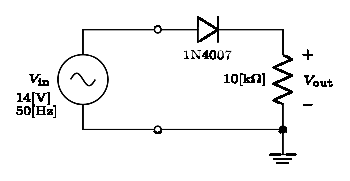
\includegraphics[scale=1.25]{02.media_onda1.eps}
\caption{Rectificador de media onda.}
\label{circuito2}
\end{figure}

Para los valores positivos del voltaje de entrada, el diodo estará polarizado
directamente, por tanto la señal de entrada caerá a través de la resistencia de
carga; mientras que con los valores negativos del voltaje de entrada, hará que
el diodo este polarizado inversamente y por tanto no circulará corriente a
traves de la carga.

\subsubsection{Onda completa con derivación central}
Este rectificador utiliza dos diodos conectados a un transformador con
derivación central como se muestra en la \textbf{figura~\ref{circuito3}}, los
voltajes entre las terminales del transformador son iguales en magnitud, pero
con diferentes fases.

\begin{figure}[!h]
\centering
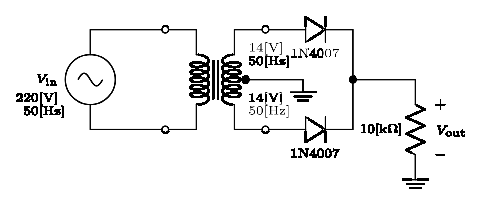
\includegraphics[scale=1.25]{03.derivacion_central1.eps}
\caption{Rectificador de onda completa con transformador de derivación central.}
\label{circuito3}
\end{figure}

La polarización directa e inversa son alternadas en cada diodo del circuito por
lo que se obtienen solo los valores positivos de cada extremo del transformador.

\subsubsection{Onda completa de puente}
Este rectificador utiliza cuatro diodos conectados como se muestra en la
\textbf{figura~\ref{circuito4}}.

\begin{figure}[!h]
\centering
\includegraphics[scale=1.25]{04.onda_completa1.eps}
\caption{Rectificador de onda completa con puente.}
\label{circuito4}
\end{figure}

Los valores positivos del voltaje de entrada polariza directamente a dos diodos
y polariza inversamente a los dos diodos restantes, mientras que los valores
negativos del voltaje hace el camino contrario por los diodos del circuito, lo
que genera la señal de onda completa con el doble de la frecuencia del voltaje
de entrada.

\subsection{Filtro}
Una vez rectificada la señal el siguiente paso es suavizar y nivelar la
corriente directa pulsante. El métdo más sencillo para lograr esto es agregar un
condensador en paralelo a La carga. El condensador se cargará durante la fase de
conducción, almacenando así energia. Cuando el diodo se apaga, el condensador
comenzará a descargarse, transfiriendo asi su energia almacenada a la carga.

Los circuitos con un filtro de $470[\mu\text{F}]$ pueden verse en la
\textbf{figura~\ref{circuito5}} para el rectificador de media onda,
\textbf{figura~\ref{circuito6}} para el rectificador de onda completa con
derivación central y \textbf{figura~\ref{circuito7}} para el rectificador de
onda completa de puente.

\begin{figure}[!h]
\centering
\includegraphics[scale=1.25]{05.media_onda2.eps}
\caption{Rectificador de media onda con filtro.}
\label{circuito5}
\end{figure}

\begin{figure}[!h]
\centering
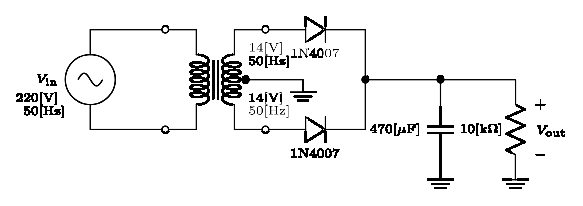
\includegraphics[scale=1.25]{06.derivacion_central2.eps}
\caption{Rectificador de onda completa con transformador de\\
derivación central y filtro.}
\label{circuito6}
\end{figure}

\begin{figure}[!h]
\centering
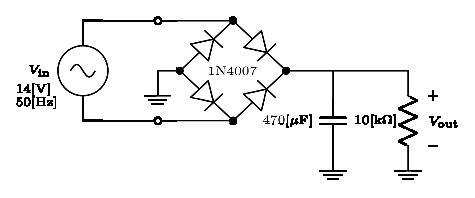
\includegraphics[scale=1.25]{07.onda_completa2.eps}
\caption{Rectificador de onda completa con puente y filtro.}
\label{circuito7}
\end{figure}

\subsection{Regulador de voltaje}
Mientras los filtros pueden reducir la fluctuación de las fuentes de
alimentación, el método más efectivo es una combinación de un filtro de entrada
con capacitor utilizado con un regulador de voltaje. Se conecta un regulador de
voltaje a la salida de un rectificador filtrado y mantiene un voltaje de salida
constante. El filtro de entrada con capacitor reduce el rizo de entrada al
regulador a un nivel aceptable. La combinación de un capacitor grande y un
regulador de voltaje ayudan a producir una excelente fuente de alimentación.

\subsubsection{Diodo \emph{Zener}}
Cuando se polariza hacia atrás con un potencial suficientemente grande, el
comportamiento normal del diodo inverso (de un interruptor abierto) cambia
abruptamente para mantener un voltaje fijo; el potencial \emph{Zener}. La
corriente a través del diodo comienza a aumentar drásticamente una vez que se
alcanza este potencial. Si se coloca un diodo \emph{Zener} a través de la salida
del rectificador filtrado, el \emph{Zener} intentará limitar el voltaje
de salida al potencial \emph{Zener}.

Para evitar el consumo excesivo y posiblemente destructivo de corriente por el
diodo \emph{Zener}, la diferencia de voltaje entre el voltaje del condensador y
el potencial \emph{Zener} se reduce a través de una resistencia limitadora de
corriente en serie. Esta resistencia limitadora establecerá la cantidad máxima
de corriente de salida. Esta corriente se divide entonces entre el diodo
\emph{Zener} y la carga.

Bajo condiciones de carga ligera, la mayor parte de esta corriente fluirá a
través del diodo \emph{Zener}. Bajo condiciones de carga pesada, la mayor parte
de la corriente será extraída por la carga con poco flujo a través del diodo
\emph{Zener}. Si la demanda de corriente de carga es demasiado pesada, no hay
corriente disponible para el diodo \emph{Zener} y deja de conducir. La
regulación se pierde y la resistencia limitadora forma un divisor de voltaje con
la carga \cite{Fiore}.

El circuito rectificador con filtro y regulador \emph{Zener} puede verse en la
\textbf{figura~\ref{circuito8}}:

\begin{figure}[!h]
\centering
\includegraphics[scale=1.25]{08.regulador1.eps}
\caption{Regulación de voltaje con diodo \emph{Zener}.}
\label{circuito8}
\end{figure}

\subsubsection{Circuitos integrados}
La mayoría de los reguladores son circuitos integrados y tienen tres terminales:
una de entrada, una de salida y una de referencia (o ajuste). Primero se filtra
la entrada al regulador con un capacitor para reducir el rizo a $<10\%$.
Típicamente, los reguladores de voltaje proporcionan una salida constante con un
alto rechazo a los rizos.

Los reguladores de tres terminales diseñados para voltajes de salida fijos
requieren sólo capacitores externos para completar la parte de regulación de la
fuente de alimentación, como se muestra la \textbf{figura~\ref{circuito9}}. El
filtrado se realiza por un capacitor de gran valor entre el voltaje de entrada y
tierra. Un capacitor de salida está conectado de la salida a tierra para mejorar
la respuesta transitoria \cite{Floyd}.

\begin{figure}[!h]
\centering
\includegraphics[scale=1.50]{09.regulador2.eps}
\caption{Regulación de voltaje con circuito integrado.}
\label{circuito9}
\end{figure}

\begin{figure}[!h]
\centering
\includegraphics[scale=1.50]{10.regulador3.eps}
\caption{Regulación de voltaje con circuito integrado negativo.}
\label{circuito9}
\end{figure}

\begin{figure}[!h]
\centering
\includegraphics[scale=1.50]{11.regulador4.eps}
\caption{Regulación de voltaje con dos circuitos integrados.}
\label{circuito9}
\end{figure}

\begin{figure}[!h]
\centering
\includegraphics[scale=1.50]{12.regulador5.eps}
\caption{Regulación de voltaje con resistencia variable.}
\label{circuito9}
\end{figure}

\section{Simulación}
Se utilizó el software \emph{Quite Universal Circuit Simulator.} versión 23.3.1
para simular los circuitos.

%   \section{Resultados}

%   \section{Conclusiones y Recomendaciones}
%   Se comprobó que los comportamientos tanto de la curva característica del diodo,
%   como de los circuitos recortadores y sustentadores, son similares en la teoría,
%   la simulación y experimentalmente.

%   Se constato que los instrumentos provistos en el laboratorio (fuentes de
%   alimentación DC, generador de funciones y osciloscopio) son vitales en el
%   análisis de circuitos y lo importante que es conocer todas las funciones que
%   proveen estos.

%   A su vez, de los componentes electrónicos de los diferentes circuitos armados
%   es crucial hacer una revisión de sus hojas de datos, para evitar que el diseño
%   exceda sus valores recomendados de funcionamiento.

\begin{thebibliography}{99}

\bibitem{Floyd}
Thomas L. Floyd (208).\\
\textbf{Dispositivos electrónicos. 8va Edición.}\\
Pearson Education\\

\bibitem{Fiore}
James M. Fiore (2017).\\
\textbf{Dispositivos semiconductores. Teoría y aplicación.}\\
Mohawk Valley Community College\\
Extraído el 12 de Octubre del 2024, de: \\
\url{https://espanol.libretexts.org/Ingenieria/Libro%3A_Dispositivos_semiconductores_-_Teor%C3%ADa_y_Aplicaci%C3%B3n_(Fiore)/03%3A_Aplicaciones_de_diodos/3.2%3A_Rectificaci%C3%B3n}

\end{thebibliography}

\end{document}

